\section{Nuclear Physics}
    \subsection{Structure of atom}
        \begin{figure}[H]
            \begin{center}
                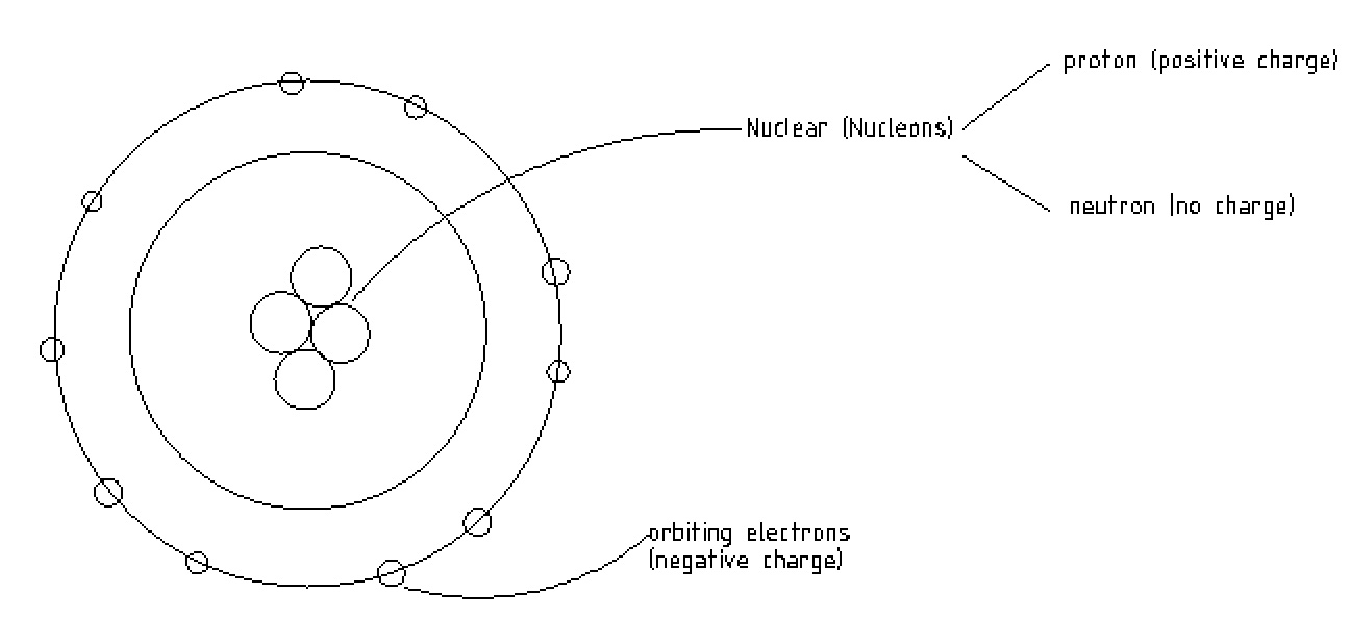
\includegraphics[height=5cm]{nuclear_charts/nuc_struct.eps}
            \end{center}
            \caption{Structure of an atom}
            \label{atom_struct}
        \end{figure}
        
        \paragraph{Isotope}
            Isotope is atoms of a same element with different number of neutrons.
        
        \paragraph{Atom symbol}
            $_Z^A X$. $A$: mass number, equal to number of protons plus number of neutrons. $Z$: atomic number, equal to number of protons.

        \paragraph{Atom mass}
            Atom mass unit, $u$, is
            \begin{align}
                1 u &= \frac{1}{12} \times \mbox{mass\ of\ one\ atom\ of\ } _6^{12} C \\
                    &= \frac{10^{-3} \mathrm{kg}}{N_A} \\
                    &= 1.66 \times 10^{-27} \mathrm{kg}
            \end{align}

            \begin{table}[H]
                \begin{center}
                    \begin{tabular}{llll}
                        \hline
                        Particle & Symbol & Mass (u) & Charge (e) \\ \hline
                        Proton & $_1^1 p$ & 1 & 1 \\
                        Neutron & $_0^1 n$ & 1 & 0 \\
                        Electron & $_{-1}^0 e$ & 0 & -1 \\
                        Positron & $_1^0 e$ & 0 & 1 \\
                        Photon & $_0^0 \gamma$ & 0 & 0 \\
                    \end{tabular}
                \end{center}
                \caption{Data of common particles}
                \label{com_part_data}
            \end{table}

    \subsection{Electronic Magnetic Spectrum}
        \paragraph{Emit spectrum}
            Low pressure gas be emitted by electricity or radiation or heat and then radiate EM wave.

            Energy of an atom is discrete. They are a specific set of values
            \begin{align}
                E_n = \frac{E_1}{n^2},\  n \in Z^+
            \end{align}

            Electrons at high energy state transit to low energy state. In this process EM wave radiated. The wave frequency is
            \begin{align}
                f = \frac{E}{h} &= \frac{E_{n1} - E_{n2}}{h} \\
                                &= \frac{\frac{E_1}{{n_1}^2} - \frac{E_1}{{n_2}^2}}{h}, \ n_1, n_2 \in Z^+
            \end{align}

        \paragraph{Absorb spectrum}
            White light (mix of light with all different frequency) lit on atom. Electrons in atom absorb some photons to gain energy and transit to high energy state. Photons that are not absorbed are observed on screen. 

            The absorbed frequency is also discrete.

            The path of energy level transittion is random.

    \subsection{Mass energy}
        \paragraph{Mass-Energy conservation}
            Einstein: When body is in high energy state, it has more mass.
            \begin{align}
                E = mc^2
            \end{align}

        \paragraph{Binding Energy}
            Binding energy is energy needed to seperate nucleons in an atom to infinity distance.

            Stability of atom is positive correlation to average binding energy per nucleon.

            \begin{figure}[H]
                \begin{center}
                    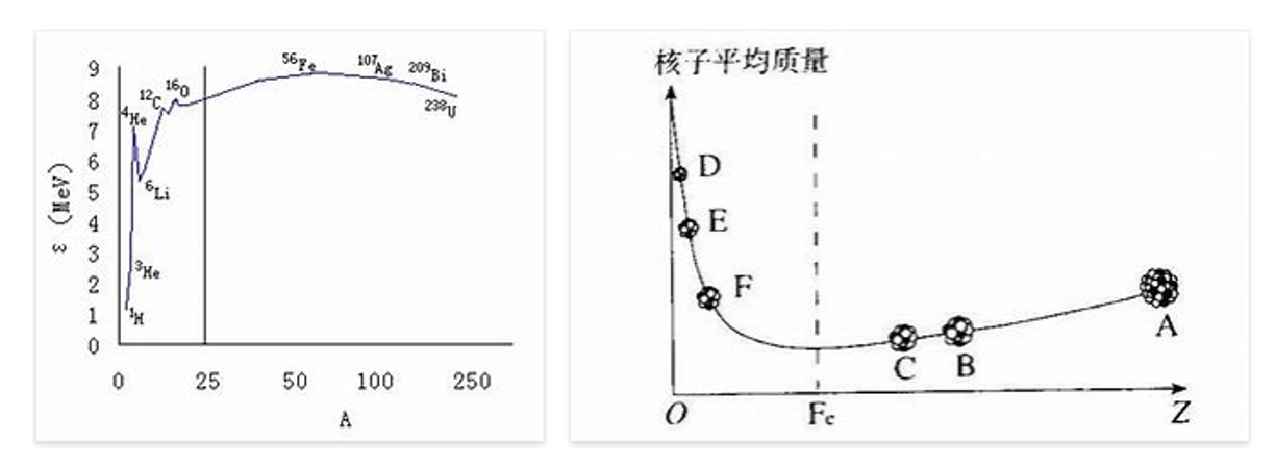
\includegraphics[height=5cm]{nuclear_charts/bind_ener.eps}
                \end{center}
                \caption{Average binding energy per nucleon and mass per nucleon against atomic number}
                \label{be_ma_an}
            \end{figure}

            Figure \ref{be_ma_an} shows the higher average binding energy is, the lower average mass. This is because mass-energy of a single nucleon is same. Thus the average binding energy $\bar{E}$ and average mass $\bar{M}$ should follow
            \begin{align}
                M c^2 + |E| = 1u c^2
            \end{align}

        \paragraph{Mass defect}
            Seperated nucleons weight more than when joined together in nucleus. This is because binding energy become smaller then mass become bigger.
    
    \subsection{Fission}
        Heavy element split to two parts and have lighter mass and release energy.

        \paragraph{Four Fundamental Forces}
            Four fundamental forces are Strong nuclear force (S), Weak nuclear force (W), electromagnetic force (M), Gravitation force (G).
            
            In order:
            \begin{align}
                S > W > M > G
            \end{align}

        \paragraph{Why more readily for heavy elements}
            The forces in nuclear are Strong force and Electromagnetic force. Strong force is attraction, electromagnetic force here is repulsion (protons have same charge).

            Relation of electromagnetic force to distance is $F \propto \frac{1}{r^2}$. Strong force is almost 0 when distance $r > 1 \times 10^{-15} \mathrm{m}$.

            Thus, for heavy elements, the distance between nucleus is bigger. Thus strong force is smaller and electromagnetic force is bigger. Thus more easily to split.

        \paragraph{Fission process for $U235$}
            Neutron collide with $U235$ $\to$ Form $U236$ $\to$ Split into two lighter atoms and release two high-energy neutrons and release energy $\to$ high-energy neutrons collide with other $U235$ atoms and chain reaction.

            Split reaction is
            \begin{align}
                U + n \to Sr + Xe + 2n
            \end{align}

    \subsection{Fusion}
        Nucleons join together and release energy.

        \paragraph{Why more readily for light elements}
            For light elements, smaller distance, higher strong force, attraction force is bigger.

            Also, according to Figure \ref{be_ma_an}, for light elements, when combine which means number of nucleons increase, the average binding energy increase, thus energy released.

        \paragraph{Process}
            Isotope of $H$ under high temperature combine and form $He$ and release energy. Released energy keep the temperature high and then chain reaction.
        
    \subsection{Differences between fission and fussion}
        \begin{table}[H]
            \begin{center}
                \begin{tabular}{l|ll}
                     & Fission & Fussion \\
                    \hline
                    Defination & Atom split & Atom combine \\
                    Natural occurrence & Not likely & In stars, e.g. Sun \\
                    Byproduct & Many radioactive particles & Little \\
                    Condition & Critical mass and high-speed neutrons & High temperature \\
                    Energy required & Low & High \\
                    Energy released & Lower & Higher \\
                    Application & Atomic bomb, power station & Hydrogen bomb, Sun
                \end{tabular}
            \end{center}
            \caption{Compare of fission and fussion}
            \label{comp_fis_fus}
        \end{table}

    \subsection{Elementary particles}
        \paragraph{Three classes of elementary particles}
            \begin{enumerate}
                \item Quarks
                \item Leptons
                \item Gauge bosons (strange particle)
            \end{enumerate}

            % Each particle has its anti-particle. For example, $_{1}^0 e$ is $_{-1}^0$'s anti particle.
        
        \paragraph{Type of quarks}

            \begin{table}[H]
                \begin{center}
                    \begin{tabular}{|l|l|l|l|l|}
                        \hline
                        Name & Symbol & Charge & Baryon number & Strangeness \\ \hline
                        up & u & \multirow{3}{*}{$+\frac{2}{3} e$} & \multirow{6}{*}{$\frac{1}{3}$} & \multirow{4}{*}{0} \\ \cline{1-2}
                        charm & c & & & \\ \cline{1-2}
                        top & t & & & \\ \cline{1-3}
                        down & d & \multirow{3}{*}{$-\frac{1}{3} e$} & & \\ \cline{1-2} \cline{5-5}
                        strange & s & & & -1 \\ \cline{1-2} \cline{5-5}
                        bottom & b & & & 0 \\ \hline
                    \end{tabular}
                \end{center}
                \caption{Type of quarks}
                \label{type_of_qk}
            \end{table}

            Hadron is particles made up of quarks or anti-quarks. It has two types:
            \begin{enumerate}
                \item Baryon, particle make up of three quarks or anti-quarks. E.g. proton, neutron
                \item Meson, particle make up of one quark and one anti-quark. E.g. Pion $\pi^0 [u, \bar{u}]$
            \end{enumerate}

        \paragraph{Type of leptons}
            \begin{table}[H]
                \begin{center}
                    \begin{tabular}{|l|l|l|l|l|l|}
                        \hline
                        Name & Symbol & Charge & $L_e$ number & $L_p$ number & $L_\gamma$ number \\ \hline
                        Electron & $e^-$ & -e & \multirow{2}{*}{+1} & \multirow{2}{*}{0} & \multirow{4}{*}{0} \\ \cline{1-3}
                        Electron neutrino & $V_e$ & 0 & & & \\ \cline{1-5}
                        Muon & $\mu^-$ & -e & \multirow{4}{*}{0} & \multirow{2}{*}{+1} &  \\ \cline{1-3}
                        Muon neutrino & $V_\mu$ & 0 & & & \\ \cline{1-3} \cline{5-6}
                        Tau & $\tau^-$ & -e & & \multirow{2}{*}{0} & \multirow{2}{*}{+1} \\ \cline{1-3}
                        Tau neutrino & $V_\tau$ & 0 & & & \\ \hline
                    \end{tabular}
                \end{center}
                \caption{Type of leptons}
                \label{type_of_lep}
            \end{table}
        
        \paragraph{Structure of common particles}
            Pion, $\pi$, type of meson, has three types:
            \begin{enumerate}
                \item $\pi^+ [u, \bar{d}]$
                \item $\pi^0 [u, \bar{u}]$
                \item $\pi^-$
            \end{enumerate}
        
            Kaon, $\kappa$, type of meson, has structure $\kappa^0 [d, \bar{s}]$

            Proton, type of baryon, $p^1[u, u, d]$

            Neutron, type of baryon, $n^0[u, d, d]$
        
        \paragraph{Conservation of lapton}
            Number of each type (family) of leptons have to be same before and after reaction.
        
        \paragraph{Muon decay}
            \begin{align}
                \mu^{\pm} \to e^{\pm} + V + \bar{V}
            \end{align}

        \paragraph{Strange particle}
            Three types: $\kappa$, $\Lambda$, $\Sigma$.

            They behave strange:
            \begin{enumerate}
                \item Always produced in pairs and decay individually
                \item They produce in fast rate and decay in slow rate
                \item When produce, must follow strangeness conservation
                \item When decay, do not need to follow strangeness conservation
            \end{enumerate}

    \subsection{Feynman Diagram}
        \begin{figure}[H]
            \begin{center}
                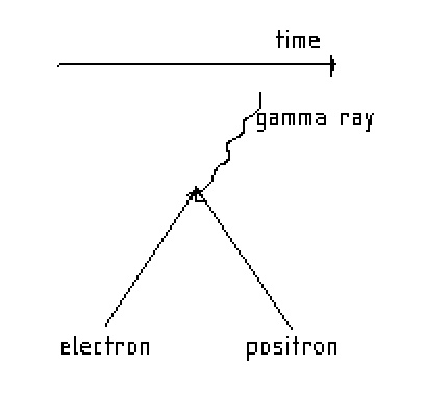
\includegraphics[height=5cm]{nuclear_charts/fym_dia.eps}
            \end{center}
            \caption{Example of Feynman Diagram}
            \label{fey_dia}
        \end{figure}

        \begin{enumerate}
            \item Particles before reaction point to one end of the line, particles after the reaction point to another end.
            \item Anti particles along negative direction of time.
            \item If Fermi particle engaged, use straight line. If photon engaged, use wave curve. If boson particle engaged, use dot line.
            \item If is boson engaged, if total charge is position, use $W^+$. If is negative, use $W^-$, if no charge, use $Z$.
        \end{enumerate}

    \subsection{Nuclear density and radius}
        \paragraph{Measure radius of nuclear}
            As shown in Figure \ref{nuc_rad_exp}, a $He$ nuclear is shoot to a gold nuclear with speed $v$ from infinity. The $He$ nuclear stops at distance $d$ from gold nuclear.

            \begin{figure}[H]
                \begin{center}
                    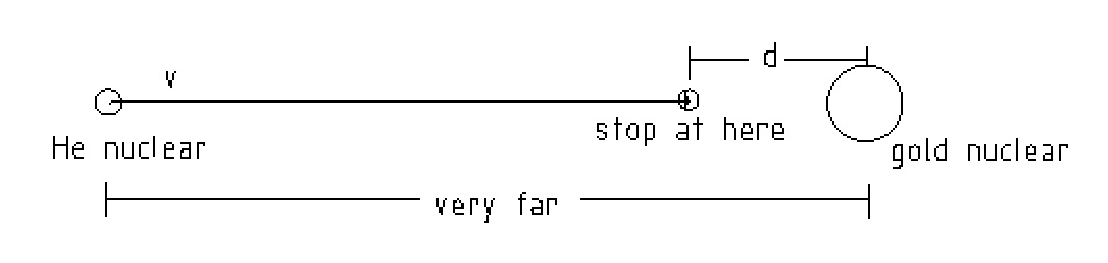
\includegraphics[height=2cm]{nuclear_charts/nuc_rad_exp.eps}
                \end{center}
                \caption{Experiment to measure nuclear radius}
                \label{nuc_rad_exp}
            \end{figure}

            Thus, 
            \begin{align}
                & \frac{1}{2} m v^2 = k \frac{2 Z e^2}{d} \\
                & \Rightarrow d = \frac{4 k Z e^2}{m v^2}
            \end{align}

            $Z$ is the atomic number of gold nuclear.

            Therefore, the radius of gold nuclear $r$
            \begin{align}
                r \approx d = \frac{4 k Z e^2}{m v^2}
            \end{align}
            
        \paragraph{Volumn of nucleon}
            Volumn of nucleus $V$ is propotional to number of nucleons $A$. Thus,
            \begin{align}
                \left\{
                    \begin{aligned}
                        V &\propto A \\
                        V &= \frac{4}{3} \pi R^3
                    \end{aligned}
                \right. &\Rightarrow 
                R^3 \propto A \\
                &\Rightarrow R \propto A^{\frac{1}{3}} \\
                &\Rightarrow R = R_0 A^{\frac{1}{3}}
            \end{align}

            $R_0$ is Fermi radius. $R_0 \approx 1.2 \times 10^{-15} \mathrm{m}$
        
        \paragraph{Nuclear density} 
            \begin{align}
                \rho = \frac{m}{V} &= \frac{A u}{\frac{4}{3} \pi (R_0 A^{\frac{1}{3}})^3} \\
                                   &= \frac{A u}{\frac{4}{3} \pi {R_0}^3 A} \\
                                   &= \frac{u}{\frac{4}{3} \pi {R_0}^3} \\
                                   &= 2 \times 10^{17} \mathrm{kg/m^3}
            \end{align}


    \subsection{Decay}
        Decay is the process a radioactive element turn into another element.

        \paragraph{Properties}
            \begin{enumerate}
                \item By random.
                \item Spontinously. Do not need trigger.
                \item Unpredictable
            \end{enumerate}

        \paragraph{Decay rate}
            $A$, the rate of decay,
            \begin{align}
                A = \frac{\mathrm{d} N}{\mathrm{d} t} \propto N
            \end{align}

        \paragraph{Decay constant}
            $\lambda$, defined as
            \begin{align}
                A = - \lambda N
            \end{align}

            The higher decay constant is, the more radioactive.

        \paragraph{Number of atoms left at time $t$}
            Let the initial number be $N_0$, the decay constant be $\lambda$.
            \begin{align}
                & \frac{\mathrm{d} N}{\mathrm{d} t} = - \lambda N \\
                & \int \frac{\mathrm{d} N}{- \lambda N} = \int \mathrm{d} t  \\
                & -\frac{1}{\lambda} \ln(N) = t + C \\
                & N = e^{- \lambda (t + C)} \\
                &= e^{-(\lambda + C)} e^{- \lambda t} \\
                & \because \mathrm{when\ } t = 0, N = N_0 \\
                & \therefore N = N_0 e^{- \lambda t}
            \end{align}

        \paragraph{Decay rate at time $t$}
            \begin{align}
                A = -\lambda N &= - \lambda N_0 e^{- \lambda t} \\
                               &= A_0 e^{- \lambda t}
            \end{align}
        
        \paragraph{Half life}
            $t_{\frac{1}{2}}$, Time needed for half of the atoms to decay.
            \begin{align}
                \frac{1}{2} N_0 &= N_0 e^{- \lambda t_{\frac{1}{2}}} \\
                - \lambda t_{\frac{1}{2}} &= \ln(\frac{1}{2}) \\ 
                                          &= - \ln(2) \\
                t_{\frac{1}{2}} &= \frac{\ln 2}{\lambda}
            \end{align}

        \paragraph{Alpha decay}
            $\alpha$ - decay, 
            \begin{align}
                _Z^A X \to _{Z-2}^{A-4} Y + _2^4 He
            \end{align}

            Energy released by mass defect only turn into $_2^4 He$'s kinetic energy. Thus the energy of $_2^4 He$ is discrete.

        \paragraph{Beta decay}
            $\beta^+$ decay:
            \begin{align}
                _Z^A X \to _{Z-1}^{A} Y + _{1}^0 e + _0^0 V_e
            \end{align}

            $\beta^-$ decay:
            \begin{align}
                _Z^A X \to _{Z+1}^{A} Y + _{-1}^0 e + _0^0 \bar{V_e}
            \end{align}

            Energy released is shared by electron and neutrino. Thus kinetic energy of each is discrete.
        
    \subsection{Pair production}
        Process that high energy gamma ray turn into a positron and an electron. Follow mass-energy conservation.

    \subsection{Annihilation}
        \begin{figure}[H]
            \begin{center}
                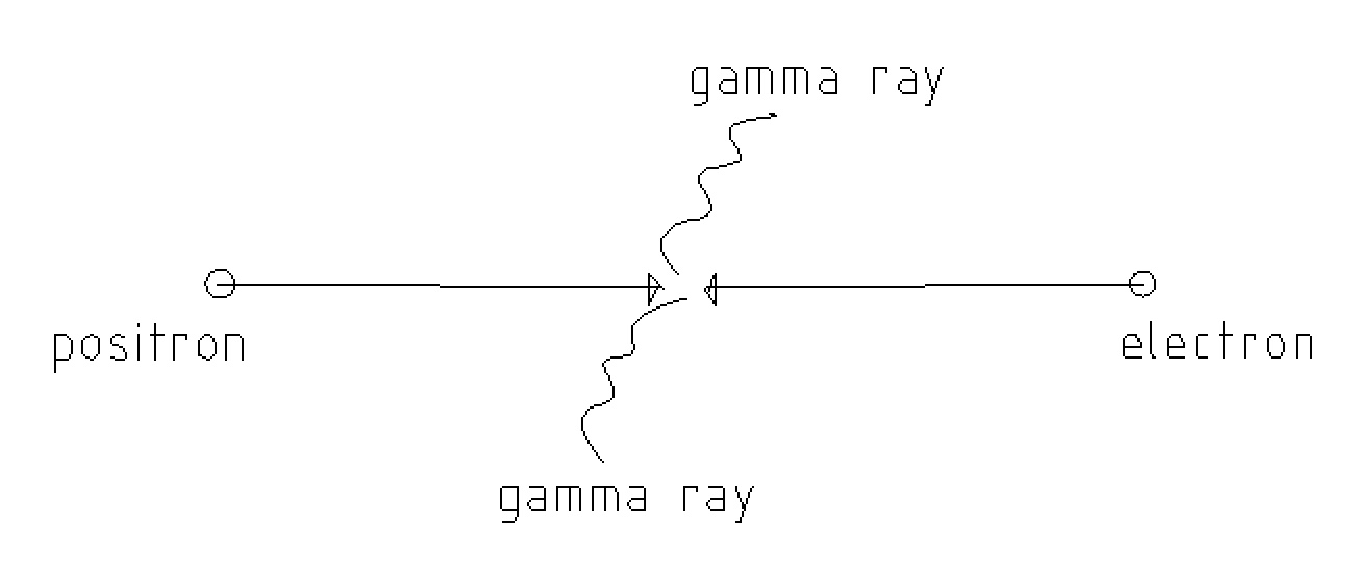
\includegraphics[height=3.5cm]{nuclear_charts/annih.eps}
            \end{center}
            \caption{Annihilation}
            \label{annih}
        \end{figure}

        Process that a positron and an electron collide and turn into gamma ray. Opposite to pair production. Follow mass-energy conservation and momentum conservation.

